\documentclass[11pt,a4paper]{article}
\usepackage[margin=3cm]{geometry}
\usepackage{tikz}
\usepackage{enumitem}
\usepackage{fancyhdr}
\usepackage{multicol}

% Minimal styling - academic worksheet appearance
\pagestyle{fancy}
\fancyhf{}
\lhead{Pattern Discovery Worksheet}
\rhead{Page \thepage}
\renewcommand{\headrulewidth}{0.4pt}
\setlength{\headheight}{14pt}

% No colors except black and gray
\definecolor{lightgray}{gray}{0.8}
\definecolor{darkgray}{gray}{0.3}

\begin{document}

% PAGE 1: Simple Title
\thispagestyle{empty}
\begin{center}
\vspace*{5cm}

{\LARGE Pattern Discovery Worksheet}

\vspace{1cm}

{\large Pre-Session Activity}

\vspace{8cm}

{\small Machine Learning for Innovation - Week 1}
\end{center}

\newpage

% PAGE 2: The Sorting Challenge
\section*{Exercise 1: The Sorting Challenge}

\noindent\textbf{Task:} Look at the dots below. Group them into categories by drawing circles around dots that belong together.

\vspace{0.5cm}

\begin{center}
\begin{tikzpicture}[scale=0.7]
% Draw border
\draw[black] (0,0) rectangle (16,10);

% Generate 100 random dots with fixed seed for reproducibility
\foreach \i in {1,...,100} {
    \pgfmathsetmacro{\xpos}{random(1,15)}
    \pgfmathsetmacro{\ypos}{random(1,9)}
    \fill[black] (\xpos,\ypos) circle (0.08);
}
% Add some clustered dots manually for better distribution
% Cluster 1 (top left)
\foreach \i in {1,...,8} {
    \pgfmathsetmacro{\xpos}{2+rand*1.2}
    \pgfmathsetmacro{\ypos}{7+rand*1.2}
    \fill[black] (\xpos,\ypos) circle (0.08);
}
% Cluster 2 (bottom right)
\foreach \i in {1,...,8} {
    \pgfmathsetmacro{\xpos}{12+rand*1.2}
    \pgfmathsetmacro{\ypos}{2+rand*1.2}
    \fill[black] (\xpos,\ypos) circle (0.08);
}
% Cluster 3 (center)
\foreach \i in {1,...,8} {
    \pgfmathsetmacro{\xpos}{8+rand*1.2}
    \pgfmathsetmacro{\ypos}{5+rand*1.2}
    \fill[black] (\xpos,\ypos) circle (0.08);
}
\end{tikzpicture}
\end{center}

\vspace{1cm}

\noindent\textbf{Questions:}

\begin{enumerate}[itemsep=0.5cm]
\item How many groups did you find? \hrulefill

\item How long did this take you? \hrulefill

\item What if there were 10,000 dots instead of 100? How long would it take? \hrulefill

\item What rule did you use to decide which dots belong together? 

\hrulefill

\hrulefill
\end{enumerate}

\newpage

% PAGE 3: The Innovation Challenge
\section*{Exercise 2: The Innovation Challenge}

\noindent\textbf{Task:} Below are 30 innovation concepts. Organize them into meaningful categories. Write the category names and list which innovations belong in each.

\vspace{0.5cm}

\begin{center}
\fbox{\parbox{0.9\textwidth}{
\begin{multicols}{2}
\begin{itemize}[label=, itemsep=0.2cm]
\item Electric transportation
\item Music streaming
\item Video communication
\item Food delivery automation
\item Digital payments
\item Remote healthcare
\item Social networking
\item Cloud storage
\item Voice assistants
\item Renewable energy
\item Online education
\item Fitness tracking
\item Smart home devices
\item Cryptocurrency
\item Ride sharing
\item Photo sharing
\item Instant messaging
\item Online marketplaces
\item Video streaming
\item Virtual reality
\item 3D printing
\item Drone delivery
\item Artificial intelligence
\item Gene editing
\item Autonomous vehicles
\item Blockchain
\item Augmented reality
\item Quantum computing
\item Internet of things
\item Sustainable packaging
\end{itemize}
\end{multicols}
}}
\end{center}

\vspace{0.5cm}

\noindent\textbf{Your Categories:}

\begin{enumerate}[itemsep=0.8cm]
\item Category 1: \hrulefill

Items: \hrulefill

\item Category 2: \hrulefill

Items: \hrulefill

\item Category 3: \hrulefill

Items: \hrulefill

\item Category 4: \hrulefill

Items: \hrulefill
\end{enumerate}

\vspace{0.5cm}

\noindent\textbf{Questions:}
\begin{enumerate}[itemsep=0.3cm]
\item Were some innovations hard to categorize? Which ones? \hrulefill

\item Could the same innovation fit multiple categories? \hrulefill

\item What if you had 5000 innovations to sort? \hrulefill
\end{enumerate}

\newpage

% PAGE 4: Exercise 3 - ML Pipeline
\section*{Exercise 3: Technical Process Sequencing}

\noindent\textbf{Task:} Below are five stages of a technical analysis process, listed alphabetically. Place them in the correct operational sequence.

\vspace{0.5cm}

\begin{center}
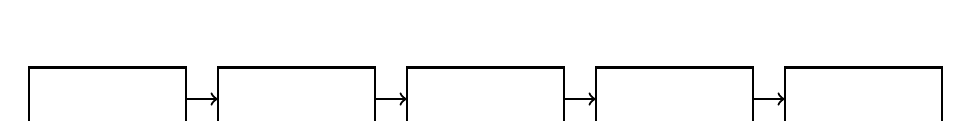
\begin{tikzpicture}[scale=0.8]
% Draw five boxes with arrows
\draw[thick] (0,0) rectangle (2.5,1);
\draw[thick,->] (2.5,0.5) -- (3,0.5);
\draw[thick] (3,0) rectangle (5.5,1);
\draw[thick,->] (5.5,0.5) -- (6,0.5);
\draw[thick] (6,0) rectangle (8.5,1);
\draw[thick,->] (8.5,0.5) -- (9,0.5);
\draw[thick] (9,0) rectangle (11.5,1);
\draw[thick,->] (11.5,0.5) -- (12,0.5);
\draw[thick] (12,0) rectangle (14.5,1);
\end{tikzpicture}
\end{center}

\vspace{0.5cm}

\noindent\textbf{Stages (alphabetical):}
\begin{itemize}[label=$\bullet$]
\item \textbf{Deploy}: Put solution into production
\item \textbf{Data}: Collect raw information
\item \textbf{Evaluate}: Test solution performance
\item \textbf{Model}: Build computational solution
\item \textbf{Preprocess}: Clean and prepare information
\end{itemize}

\vspace{0.5cm}

\noindent\textbf{Questions:}
\begin{enumerate}[itemsep=0.5cm]
\item Why must this sequence be followed strictly? \hrulefill

\hrulefill

\item What happens if you skip the second step? \hrulefill

\item At which step do errors become most costly? \hrulefill

\item Which step requires the most computational resources? \hrulefill

\item Can any two steps be performed simultaneously? \hrulefill
\end{enumerate}

\newpage

% PAGE 5: Exercise 4 - Design Thinking Pipeline
\section*{Exercise 4: Human-Centered Process Sequencing}

\noindent\textbf{Task:} Below are five stages of a human-centered problem-solving process, listed alphabetically. Arrange them in logical sequence.

\vspace{0.5cm}

\begin{center}
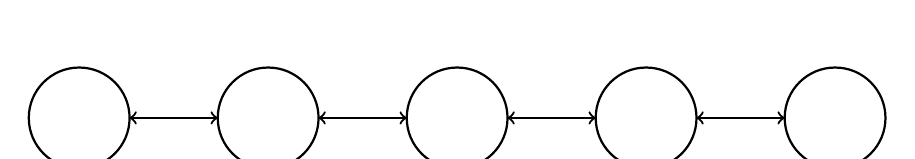
\begin{tikzpicture}[scale=0.8]
% Draw five circles with bidirectional arrows
\draw[thick] (0,0) circle (0.8);
\draw[thick,<->] (0.8,0) -- (2.2,0);
\draw[thick] (3,0) circle (0.8);
\draw[thick,<->] (3.8,0) -- (5.2,0);
\draw[thick] (6,0) circle (0.8);
\draw[thick,<->] (6.8,0) -- (8.2,0);
\draw[thick] (9,0) circle (0.8);
\draw[thick,<->] (9.8,0) -- (11.2,0);
\draw[thick] (12,0) circle (0.8);
\end{tikzpicture}
\end{center}

\vspace{0.5cm}

\noindent\textbf{Stages (alphabetical):}
\begin{itemize}[label=$\bullet$]
\item \textbf{Define}: Articulate the problem
\item \textbf{Empathize}: Understand user needs
\item \textbf{Ideate}: Generate potential solutions
\item \textbf{Prototype}: Build preliminary solution
\item \textbf{Test}: Validate with users
\end{itemize}

\vspace{0.5cm}

\noindent\textbf{Questions:}
\begin{enumerate}[itemsep=0.5cm]
\item Unlike the technical process, why are the arrows bidirectional? \hrulefill

\hrulefill

\item Which stage requires the most human interaction? \hrulefill

\item Can you begin at stage 3? Why or why not? \hrulefill

\hrulefill

\item How does stage 1 inform stage 2? \hrulefill

\item Why might you return to stage 1 after stage 5? \hrulefill
\end{enumerate}

\newpage

% PAGE 6: Exercise 5 - Pipeline Convergence
\section*{Exercise 5: Methodological Integration}

\noindent\textbf{Task:} Identify how each technical stage could inform the corresponding human-centered stage.

\vspace{0.5cm}

\begin{center}
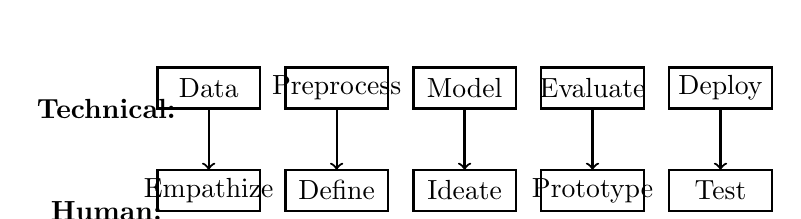
\begin{tikzpicture}[scale=0.65]
% Technical Pipeline
\node at (-1, 2) {\textbf{Technical:}};
\draw[thick] (0,2) rectangle (2,2.8) node[midway] {Data};
\draw[thick] (2.5,2) rectangle (4.5,2.8) node[midway] {Preprocess};
\draw[thick] (5,2) rectangle (7,2.8) node[midway] {Model};
\draw[thick] (7.5,2) rectangle (9.5,2.8) node[midway] {Evaluate};
\draw[thick] (10,2) rectangle (12,2.8) node[midway] {Deploy};

% Arrows between pipelines
\draw[thick,->] (1,2) -- (1,0.8);
\draw[thick,->] (3.5,2) -- (3.5,0.8);
\draw[thick,->] (6,2) -- (6,0.8);
\draw[thick,->] (8.5,2) -- (8.5,0.8);
\draw[thick,->] (11,2) -- (11,0.8);

% Human Pipeline
\node at (-1, 0) {\textbf{Human:}};
\draw[thick] (0,0) rectangle (2,0.8) node[midway] {Empathize};
\draw[thick] (2.5,0) rectangle (4.5,0.8) node[midway] {Define};
\draw[thick] (5,0) rectangle (7,0.8) node[midway] {Ideate};
\draw[thick] (7.5,0) rectangle (9.5,0.8) node[midway] {Prototype};
\draw[thick] (10,0) rectangle (12,0.8) node[midway] {Test};
\end{tikzpicture}
\end{center}

\vspace{0.5cm}

\noindent\textbf{Analysis Questions:}
\begin{enumerate}[itemsep=0.5cm]
\item How does "Data" inform "Empathize"? \hrulefill

\hrulefill

\item How does "Define" constrain "Preprocess"? \hrulefill

\hrulefill

\item Where is the strongest connection? Why? \hrulefill

\hrulefill

\item Where is the weakest connection? Why? \hrulefill

\hrulefill

\item What is lost if these pipelines operate independently? \hrulefill

\hrulefill

\item Identify one feedback loop between pipelines: \hrulefill

\hrulefill
\end{enumerate}

\newpage

% PAGE 7: Reflection
\section*{Reflection: Methodological Synthesis}

\vspace{0.5cm}

\noindent Synthesize your observations from all exercises:

\vspace{0.8cm}

\begin{enumerate}[itemsep=1cm]
\item Compare the rigidity of technical versus human-centered processes:

\hrulefill

\hrulefill

\hrulefill

\item Explain why iteration is essential in one pipeline but problematic in the other:

\hrulefill

\hrulefill

\hrulefill

\item Identify the primary constraint in each pipeline:

\hrulefill

\hrulefill

\item Describe how quantitative and qualitative methods complement each other:

\hrulefill

\hrulefill

\hrulefill

\item What is the epistemological difference between "Model" and "Ideate"?

\hrulefill

\hrulefill

\hrulefill

\item Propose how automation could enhance human-centered design:

\hrulefill

\hrulefill

\hrulefill
\end{enumerate}

\vspace{1.5cm}

\noindent\rule{\textwidth}{0.4pt}

\vspace{0.5cm}

\noindent\textit{In our first session, we will explore how these two pipelines converge to create innovation opportunities through the systematic application of machine learning to design thinking challenges.}

\end{document}